\chapter{Introdução}

\section{Âmbito do Projeto}

\textbf{GrabATable – Plataforma de gestão de reservas de restaurantes}

A plataforma GrabATable consiste num sistema de gestão de reservas para restaurantes que combina dois mecanismos complementares: reservas antecipadas e gestão de fila de espera em tempo real para clientes sem reserva.

\subsection{Problema Identificado}

Os restaurantes que gerem reservas em papel, por telefone ou em sistemas isolados não conseguem conciliar as reservas com a afluência de clientes sem marcação. O resultado é sobrelotação, esperas imprevisíveis e uma má experiência tanto para quem reservou como para quem chegou sem reserva.

\subsection{Solução Proposta}

O cliente pode reservar mesa para uma data e hora, ou, ao chegar sem reserva, entrar numa fila virtual e acompanhar o tempo estimado. O sistema cruza reservas confirmadas, tempo médio de refeição e fila ativa para calcular a estimativa e avisa o
cliente quando a mesa estiver quase disponível. O sistema cruza continuamente a disponibilidade de mesas (reservas confirmadas, tempo médio de refeição e fila de espera atual) para calcular estimativas dinâmicas, notificando o cliente quando a mesa estiver próxima de ficar disponível.

\subsection{Inovação}

A fila de espera não é uma lista à parte: é um recurso gerido em conjunto com as
reservas, o que justifica uma arquitetura de microsserviços~\cite{newman,lewisfowler} (cálculo de espera a partir de
vários domínios, quase em tempo real).

\section{Público-Alvo e Tarefa Principal}

Há três perfis de utilizador, cada um com uma tarefa principal diferente.

\begin{table}[H]
    \centering
    \renewcommand{\arraystretch}{1.3}
    \begin{tabularx}{\textwidth}{@{}l X X X@{}}
        \toprule
        \textbf{Perfil} & \textbf{Quem é} & \textbf{Tarefa Principal} & \textbf{Contexto de uso} \\
        \midrule

        Cliente &
        Adultos dos 18 aos 55 anos, familiarizados com o uso do telemóvel &
        Reservar mesa ou entrar na fila e saber quanto tempo vai esperar &
        Telemóvel, muitas vezes a caminho do restaurante \\
        \midrule

        Gestor &
        Gerente ou responsável de sala de um restaurante &
        Gerir reservas, mesas e fila durante o serviço &
        Tablet ou computador, sob pressão de tempo \\
        \midrule

        Administrador &
        Equipa responsável pela plataforma &
        Configurar restaurantes, utilizadores e políticas globais &
        Computador, de forma pontual \\

        \bottomrule
    \end{tabularx}
    \caption{Público-alvo e tarefa principal}
    \label{tab:publico-alvo}
\end{table}

A tarefa central de todo o sistema é \textbf{garantir mesa sem surpresas:} o cliente sabe sempre se tem mesa e quando, e o gestor vê a ocupação e a fila num só ecrã.

\section{Objetivos}
O principal objetivo do projeto GrabATable é desenvolver uma plataforma de gestão de reservas e filas de espera para restaurantes, permitindo melhorar a organização da ocupação do estabelecimento e proporcionar aos clientes uma experiência mais previsível e eficiente.

A plataforma pretende centralizar a gestão de reservas antecipadas e de clientes sem reserva, utilizando a informação sobre a disponibilidade das mesas, reservas existentes, fila de espera e tempo médio de permanência para disponibilizar estimativas de espera atualizadas em tempo real.

Para concretizar o objetivo geral, o sistema deverá:
\begin{itemize}
    \item Permitir aos clientes consultar a disponibilidade de mesas e efetuar reservas para uma data e hora específicas;
    \item Permitir aos clientes entrar numa fila de espera virtual quando não possuem reserva;
    \item Disponibilizar ao cliente uma estimativa do tempo de espera, atualizada de acordo com a ocupação e rotatividade do restaurante;
    \item Notificar o cliente quando a sua mesa estiver próxima de ficar disponível;
    \item Permitir aos gestores dos restaurantes visualizar e gerir as reservas existentes;
    \item Permitir aos gestores gerir a fila de espera em tempo real;
    \item Permitir registar a chegada dos clientes, bem como situações de falta de comparência;
    \item Permitir aos gestores configurar e atualizar o estado das mesas do restaurante;
    \item Apoiar a distribuição dos clientes pelas mesas disponíveis de forma organizada;
    \item Permitir aos administradores gerir os restaurantes registados na plataforma;
    \item Permitir a configuração de políticas gerais da plataforma, como regras de falta de comparência e parâmetros relacionados com o tempo médio de refeição;
    \item Centralizar a informação relacionada com reservas, mesas e filas de espera numa única plataforma;
    \item Garantir uma interface simples e intuitiva, adequada aos diferentes perfis de utilizador;
    \item Melhorar a previsibilidade dos tempos de espera e reduzir situações de sobrelotação ou má gestão da capacidade do restaurante.
\end{itemize}

\section{Sistema Visual}\label{sec:sistema-visual}

A identidade combina um tom acolhedor, ligado à restauração, com interfaces limpas e legíveis.

\subsection{Logótipo}

\textit{Wordmark} "GrabATable" em tipografia arredondada, com o "A" no centro. O logótipo apresenta uma identidade visual moderna, minimalista e acolhedora, associada ao setor da restauração e à reserva de mesas em restaurantes. Combina um símbolo gráfico facilmente reconhecível com um nome de marca de grande destaque, utilizando uma paleta de cores que transmite frescura, confiança e proximidade.

\begin{figure}[H]
    \centering
    
\includegraphics[width=0.4\linewidth]{images/Logo.png}
    \caption{Logótipo}
    \label{fig:1}
\end{figure}

\subsection{Paleta Cromática}

A paleta cromática do GrabATable foi definida de forma a transmitir uma identidade visual simples, elegante e associada ao contexto de restauração.
A paleta cromática foi gerada com a ferramenta Coolors~\cite{coolors}.

\begin{figure}[H]
    \centering
    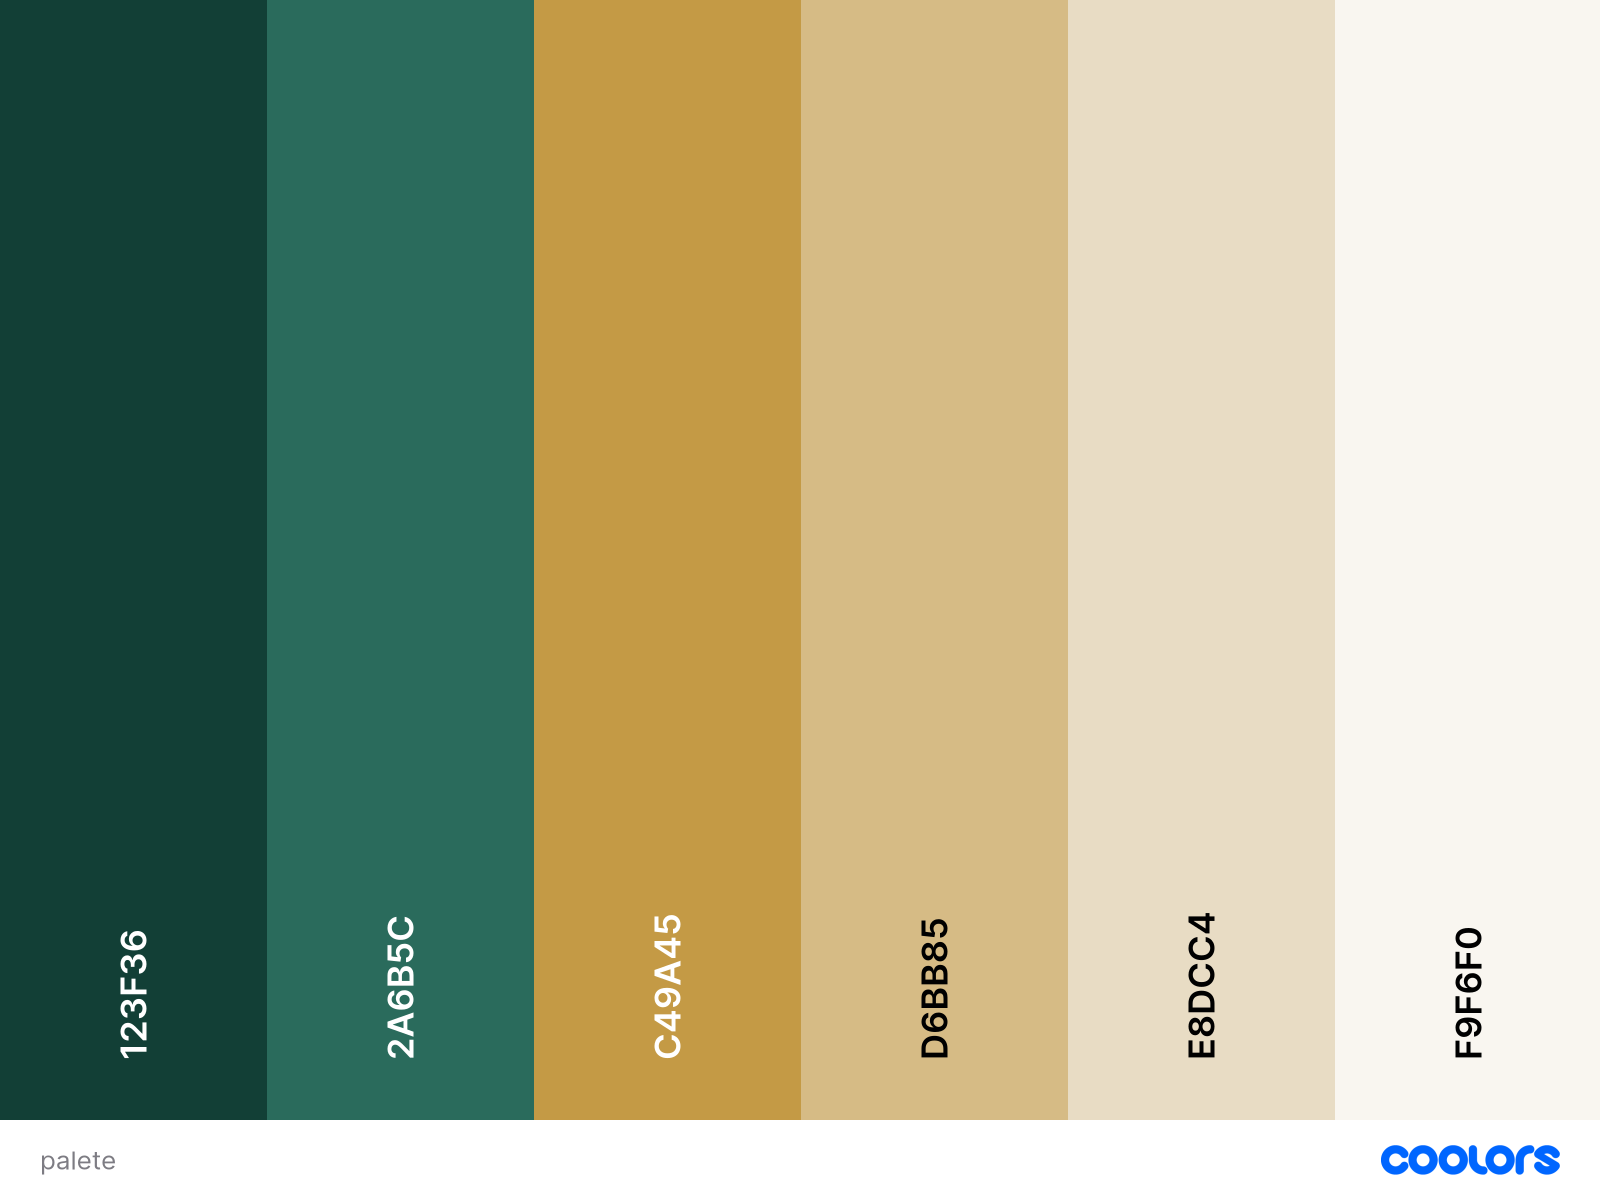
\includegraphics[width=0.6\linewidth]{images/paleta.png}
    \caption{Paleta Cromática}
    \label{fig:2}
\end{figure}

\begin{table}[H]
    \centering
    \renewcommand{\arraystretch}{1.3}
    \begin{tabularx}{\textwidth}{@{}l X X X@{}}
        \toprule
        \textbf{Papel} & \textbf{Nome} & \textbf{Hex} & \textbf{Uso} \\
        \midrule

        Primária &
        Verde floresta &
        \#123F36 &
        Texto principal, títulos, cabeçalhos \\
        \midrule

        Secundária &
        Verde &
        \#2A6B5C &
        Botões principais, ligações, estado confirmado \\
        \midrule

        Destaque &
        Ouro &
        \#C49A45 &
        Fila de espera, ícones e realces \\
        \midrule

        Apoio &
        Areia &
        \#D6BB85 &
        Etiquetas e fundos de realce, só com texto escuro \\
        \midrule

        Superfície &
        Bege &
        \#E8DCC4 &
        Cartões, separadores e campos \\
        \midrule

        Fundo &
        Creme &
        \#F9F6F0 &
        Fundo das páginas \\
        \midrule

        Erro &
        Vermelho &
        \#B91C1C &
        Erros e cancelamentos \\

        \bottomrule
    \end{tabularx}
    \caption{Paleta cromática}
    \label{tab:paleta-cromatica}
\end{table}

\subsection{Tipografia}

Títulos em \textit{Poppins} \textit{SemiBold} e texto corrido em Inter Regular, ambas gratuitas (Google \textit{Fonts}~\cite{googlefonts}). Escala: 32, 24, 20 px para títulos; 16 px para texto; 14 e 12 px para apoio. Altura de linha 1,5 no texto corrido.

\subsection{Grelha e Margens}

\subsubsection{Escala de espaçamento}

\begin{itemize}
    \item \textbf{4–8 px:} entre ícone e texto, ou dentro de componentes;
    \item \textbf{12–16 px:} \textit{padding} de botões e cartões, e espaço entre campos de formulário;
    \item \textbf{24–32 px:} entre grupos de conteúdo;
    \item \textbf{48–80 px:} entre secções da página.
\end{itemize}

\subsubsection{Grelha de colunas por tipo de dispositivo}

\begin{table}[H]
    \centering
    \renewcommand{\arraystretch}{1.1}
    \begin{tabularx}{\textwidth}{@{}l L L L L@{}}
        \toprule
        \textbf{Dispositivo} & \textbf{Largura do ecrã} & \textbf{Colunas} & \textbf{Margem lateral} & \textbf{\textit{Gutter} (Espaço entre colunas)} \\
        \midrule
        Telemóvel  & $<$ 600 px     & 4  & 16 px         & 16 px \\
        \midrule
        Tablet     & 600-839 px    & 8  & 24 px         & 24 px \\
        \midrule
        Computador & $\geq$ 1200 px & 12 & 32 px ou mais & 24--32 px \\
        \bottomrule
    \end{tabularx}
    \caption{Grelha responsiva por tipo de dispositivo}
    \label{tab:grelha}
\end{table}



\subsection{Componentes Principais}

\begin{itemize}
    \item Botão primário, secundário e de texto, com estados normal, foco, premido e desativado;
    \item Cartão de restaurante (foto, nome, cozinha, disponibilidade);
    \item Seletor de data, hora e número de pessoas;
    \item Indicador de tempo de espera, com minutos e posição na fila;
    \item Etiqueta de estado da reserva (pendente, confirmada, cancelada, não comparência);
    \item Barra de navegação por perfil e menu lateral de gestão;
    \item Tabela de gestão com filtros e ações por linha;
    \item Notificações e alertas de erro em formulários.
\end{itemize}

\subsection{Acessibilidade Cromática}

O texto escuro sobre fundos claros e o texto claro sobre verde passam o nível AA da \textit{WCAG} 2.1~\cite{wcag} (mínimo 4,5:1 para texto normal); o ouro e a areia falham com texto claro ou verde. Os rácios foram calculados com a fórmula de luminância relativa da \textit{WCAG}.

\begin{table}[H]
    \centering
    \renewcommand{\arraystretch}{1.3}
    \begin{tabularx}{\textwidth}{@{}l X X@{}}
        \toprule
        \textbf{Texto / fundo} & \textbf{Rácio} & \textbf{AA (4,5:1)} \\
        \midrule

        Verde floresta / Creme &
        10,88 &
        Passa \\
        \midrule

        Verde floresta / Bege &
        8,64 &
        Passa \\
        \midrule

        Verde floresta / Areia &
        6,32 &
        Passa \\
        \midrule

        Vermelho / Creme &
        6,00 &
        Passa \\
        \midrule

        Verde / Creme &
        5,80 &
        Passa \\
        \midrule

        Verde / Bege &
        4,61 &
        Passa \\
        \midrule

        Verde floresta / Ouro &
        4,50 &
        Passa, por margem mínima \\
        \midrule

        Verde / Areia &
        3,37 &
        Falha \\
        \midrule

        Branco / Ouro &
        2,61 &
        Falha \\
        \midrule

        Creme / Ouro &
        2,42 &
        Falha \\
        \midrule

        Verde / Ouro &
        2,40 &
        Falha \\
        \midrule

        Ouro / Bege &
        1,92 &
        Falha \\

        \bottomrule
    \end{tabularx}
    \caption{Acessibilidade cromática}
    \label{tab:acessibilidade-cromatica}
\end{table}

\subsubsection{Problema encontrado}

A legenda do diagrama usa texto branco sobre amarelo (1,84), verde (2,28) e vermelho (3,76), e todas falham. Correção: texto Carvão
sobre o amarelo (7,98) e sobre o verde, ou substituir os círculos por etiquetas com texto.

\subsubsection{Regras adotadas}

\begin{itemize}
    \item O ouro nunca leva texto claro nem verde por cima; com ele usa-se Verde floresta (4,50:1, no limite);
    \item Ouro sobre Creme dá 2,42:1, abaixo dos 3:1 exigidos a ícones e bordas, pelo que estes usam Verde (5,80:1) e o ouro fica só como realce;
    \item A cor nunca é o único meio de informação: estados de reserva e fila têm sempre texto e ícone;
    \item Foco de teclado visível, com contorno de 2 px em Verde.
\end{itemize}